\documentclass[runningheads]{llncs}

\usepackage{cite}
\usepackage{amsmath,amssymb,amsfonts}
\usepackage{algorithmic}
\usepackage{graphicx}
\usepackage{textcomp}
\usepackage{xcolor}

\usepackage{color, colortbl}
\usepackage{subcaption}
\captionsetup{compatibility=false}
\usepackage{listings}
\usepackage{url}
\usepackage{epsfig}
\usepackage{multicol}


\definecolor{myred}{RGB}{248, 118, 109}
\definecolor{mygreen}{RGB}{0, 186, 56}
\definecolor{myblue}{RGB}{97, 156, 255}

\renewcommand{\arraystretch}{1.4}

\begin{document}

%\title{DetGen: Data generation to bridge the "semantic gap" in network intrusion detection}
\title{Contribution Title\thanks{Supported by organization x.}}
%
%\titlerunning{Abbreviated paper title}
% If the paper title is too long for the running head, you can set
% an abbreviated paper title here
%
\author{First Author\inst{1}\orcidID{0000-1111-2222-3333} \and
Second Author\inst{2,3}\orcidID{1111-2222-3333-4444} \and
Third Author\inst{3}\orcidID{2222--3333-4444-5555}}
%
\authorrunning{F. Author et al.}
% First names are abbreviated in the running head.
% If there are more than two authors, 'et al.' is used.
%
\institute{Princeton University, Princeton NJ 08544, USA \and
Springer Heidelberg, Tiergartenstr. 17, 69121 Heidelberg, Germany
\email{lncs@springer.com}\\
\url{http://www.springer.com/gp/computer-science/lncs} \and
ABC Institute, Rupert-Karls-University Heidelberg, Heidelberg, Germany\\
\email{\{abc,lncs\}@uni-heidelberg.de}}
%
\maketitle   

%\pagebreak
\begin{abstract}

We introduce DetGen, \textcolor{red}{tool} that generates traffic to \textcolor{red}{improve} the ability to probe and understand model behaviour in data-driven network intrusion detection, and help explain the corresponding decisions made by a model. 
DetGen operates under a \textcolor{red}{new} design paradigm based on containerisation and reproducibility in order to closely controlling different factors that influence generated network traffic and providing cross-linkage information between captured traffic and these factors.
In this work, we \textcolor{red}{demonstrate} how DetGen operates. 
\begin{itemize}

\item We examine how well DetGen is able to control different types of traffic characteristics, and compare the corresponding \textcolor{red}{determinism} to common VM-based traffic generation setups.

\item We also examine the performance of DetGen \textcolor{red}{in the other direction}, namely the ability to generate traffic with realistic levels heterogeneity, and compare the results against those observed in existing artificially generation NID-datasets.

\item We present an exemplary dataset that is suitable for a broad probing of models trained on the CICIDS-17 dataset, as it mirrors its range of protocols and attacks.

\item We demonstrate the extensive probing of an LSTM-based anomaly detection model with this dataset, and demonstrate how to lower false-positives effectively by understanding where the model fails to process particular traffic structures correctly.

\end{itemize}
\end{abstract}



%\pagebreak


\section{Introduction}

In this work, we introduce a new traffic generation \textcolor{red}{tool} that \textcolor{red}{improves} the ability to probe and understand model behaviour in data-driven network intrusion detection, and help explain the corresponding decisions made by a model. 


in network intrusion detection by closely controlling different factors that influence generated network traffic and providing cross-linkage information between captured traffic and these factors. Our design relies on a composition of containers to enable capturing traffic directly from programs that run in an isolated and reproducible manner. Rather than simulating the large-scale behaviour of users in a realistic way, we aim to generate small-scale traffic scenarios that contain true interactions between software components in a realistic way to enable researchers a better understanding of particular traffic events. 



Data-driven traffic analysis and attack detection is a centrepiece of network intrusion detection research, and the idea of training systems on large amounts of network traffic to develop a generalised notion of bad and benign behaviour appears  like the solution to cyber-threats and has received \textit{tremendous} attention in the academic literature. However, existing datasets fall short on available ground-truth information about particular traffic characteristics that could affect model performance. Furthermore, the generation process for synthetic traffic usually does not provide sufficient structural nuances to explore the behaviour of model .\textcolor{red}{insert citation}


%However, operational deployment is dominated by systems relying on more restrictive attack signatures. Already in 2010 Paxson and Sommer \cite{sommer2010outside} have identified a number of \textcolor{red}{issues} that are summarised as an overall lack of connection between the nature of intrusion detection data and the applied data-driven detection systems, something the authors call the `semantic gap'. These findings have since then been confirmed by other authors such as Harang \cite{harang2014bridging} in 2014 or by Liu et al. in 2019 \cite{liu2019machine}.

%Among others, these issues include (1) fundamental difficulties for conducting sound evaluation of detection models \textcolor{red}{and a (2) lacking perspective of a network operator that handles alerts,} that result in a (3) semantic gap between the development of detection models and the structural and operational nature of network traffic and intrusion detection. 


%As an example, results in  were not achieved solely by training models on large annotated datasets, but have been reliant on specialised datasets that highlight and label speech structures such as emotions (RAVDESS dataset), noise, or accents 

%between results and their operational interpretation.

Machine-learning breakthroughs in other fields have often been reliant on a precise understanding of data structure and corresponding descriptive labelling to develop more suitable models.
%As an example, results in \textit{automatic speech recognition (ARS)} were not achieved by immediately training then state-of-the-art models on large annotated datasets. 
Initial models in \textit{automatic speech recognition (ASR)} for example were reliant on highly sanitised and structured speech snippets in order to isolate low-level structures such as phonemes or time-warping, before the understanding of these structures lead to the success of more layered models of feed-forward and recurrent neural networks and more recently fully end-to-end trained models. Lately, datasets that contain labelled specialised speech characteristics enable researchers to better understand ASR weak points such as emotional speech (RAVDESS), accents (Speech Accent Archive), or background noise (Urban Sound Dataset).

In a similar fashion, several approaches to enhance the way information is collected and presented have been successful in improving understanding between data and detection systems in different areas of information security. Virtual machine introspection monitors and analyses the runtime state of a system-level VM, and the inclusion of threat reports to create behavioural feature labels enriches the way executables are described \cite{smith2020mind}. Recently, data provenance tools aim to improve the representation of system executions \cite{barre2019mining} over traditional logs. 

However, such efforts have not been made in network intrusion detection yet, with the current quasi-benchmark datasets paying more attention to the inclusion of a wide variety of attacks rather than the close control and detailed documentation of the generated traffic. Data containing ground-truth on the traffic generation process to link observable structures with corresponding computational activities is rare, which has so far lead researchers to predominantly apply a number of ML-models to traffic datasets in the hope of edging out competitors. %In-depth analyses regarding which traffic characteristics lead to inaccurate predictions or cause a model to misbehave,
This overall lack of connection between the nature of intrusion detection data and the applied data-driven detection systems has been identified as a `semantic gap' by Paxson and Sommer \cite{sommer2010outside}, and is seen to be partly responsible for the lack of success machine-learning had in network intrusion detection. This claim has been supported and partly extended by Harang \cite{harang2014bridging} in 2014 and by Liu et al. in 2019 \cite{liu2019machine}.

%By moving from virtual machines to containers, we enable the scalable, modular, and dynamic creation of network traffic datasets. Since containers can be arranged in complex settings with a few commands, it is a lot easier with containers to script a variety of network activities thus increase the heterogeneity and realism of the generated data.

 
%We propose a novel design paradigm that makes generation of network traffic and corresponding attacks significantly more flexible and offers a \textcolor{red}{new level} of insight and reproducibility for traffic micro-structures through the use of containerisation. 
This work provides the following contributions:



In this work, we \textcolor{red}{demonstrate} how DetGen operates. 
\begin{enumerate}
\item We propose DetGen, a framework based on a novel design paradigm for generating reproducible small-scale traffic structures with ground-truth labels that contain extensive information about the computational interactions behind it. 

\item We explain how DetGen enables accurate and \textcolor{red}{quasi-deterministic} control over traffic characteristics as well as corresponding ground truth informtation, and compare the design advantages to traditional generation set-ups.

\item We examine how well DetGen is able to control different types of traffic characteristics, and compare the corresponding \textcolor{red}{determinism} to common VM-based traffic generation setups.

\item We also examine the performance of DetGen \textcolor{red}{in the other direction}, namely the ability to generate traffic with realistic levels heterogeneity, and compare the results against those observed in existing artificially generation NID-datasets.

\item We present an exemplary dataset that is suitable for a broad probing of models trained on the CICIDS-17 dataset, as it mirrors its range of protocols and attacks.

\item We demonstrate the extensive probing of an LSTM-based anomaly detection model with this dataset, and demonstrate how to lower false-positives effectively by understanding where the model fails to process particular traffic structures correctly.
\end{enumerate}

This framework is openly accessible for researchers and allows for straightforward customization.


\subsection{Outline}

%The remainder of the paper is organized as follows. Section \ref{Sec:Motivation} discusses the necessity for probing to validate and understand ML-models, and our methodology of using traffic micro-structure control for model probing. In Sections \ref{Sec:Improvedtrafficsep} and \ref{Sec:Refining} we demonstrate how to perform model probing and implement corresponding design improvements on two network intrusion detection models. Section \ref{Sec:Conclusion}  concludes the results and discusses limitations of our work and directions for future work.

\section{Motivation and Methodology}\label{Sec:Motivation}

%\subsection{Motivation}

Scientific machine learning model development requires both \textbf{model evaluation}, in which the overall predictive quality of a model is assessed to identify the best model, as well as \textbf{model validation}, in which the behaviour and limitations of a model is assessed through targeted \textbf{model probing}. Model validation is essential to understand how particular data structures are processed, and enables researchers to develop their models accordingly. Data generation tools for rapid model probing in other domains such as the \textit{What-If tool} \cite{wexler2019if} underline the importance of model validation.


\begin{figure}
\centering
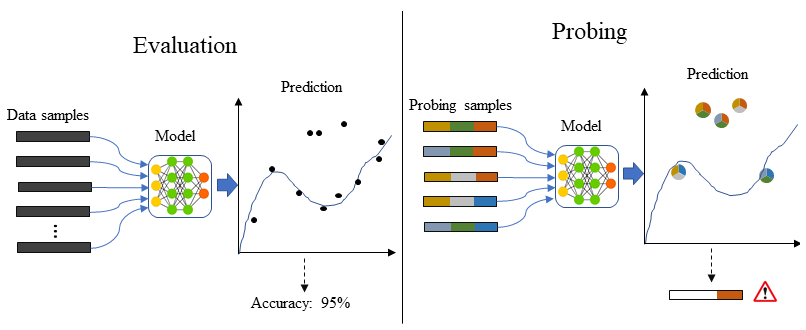
\includegraphics[width=\textwidth]{images/Eva_Prob.png}
\caption{Comparison between numerical model evaluation and model probing with specifically controlled data characteristics, indicated as colours.}
\end{figure}

Assume the following problem: You are designing a traffic classifier for a specific setting, which is generating a significant amount of misclassifications, which have a non-obvious origin. Existing real-world or synthetic datasets do not contain the necessary information to describe the misclassified traffic events, which makes it very tedious to compare identify particular features responsible for the misclassification. 

DetGen is designed to provide traffic with the necessary ground-truth information to allow effective association of model processing behaviour with corresponding traffic characteristics. Traffic is generated with exact control and monitoring over the conducted communication activity as well as various traffic \textcolor{red}{micro-structures} such as network failures or specific implementations.

Below, we provide a use-case to demonstrate how ground-truth information and traffic micro-structure-control enables effective model probing:

%\section{Use-cases}
\subsection{Improved traffic separation for a classifier with congestion level information}\label{Sec:Improvedtrafficsep}


%Possible title: \textbf{Exploring the effect of rare events to model performance}
%Our first example looks at how descriptive ground truth information on traffic characteristics can improve a
In this example we improve the design of a traffic classification model through the analysis of data separation in dependence of different traffic features. For this, we use a recent traffic classification model by Hwang et al. \cite{hwang2019lstm} as an example, which aims at distinguishing various types of malicious activity from benign traffic. The model achieved some of the highest detection rates of packet-based classifiers in a recent survey \cite{tahaei2020rise}.
The model classifies connections on a packet-level using a \textit{Long-short-term memory} (LSTM) network \footnote{a deep learning design for sequential data}, and is claimed to achieve detection and false-positive (FP) rates of \textbf{99.7\%} and \textbf{0.03\%} respectively. 


We train a model on a set of different HTTP-activities in order to detect SQL-injections. Rather than providing an accurate and realistic detection setting, this example shows how traffic information can be linked to model failures and slumping performance. We use real-world HTTP-traffic from the \textit{CAIDA anonymized traffic traces} \cite{walsworth2015caida} as background traffic (85\% of connections) and add SQL-injection attack traffic (7.5\%) as well as different HTTP-activities for probing (7.5\%). In total, we use 50,000 connections for training the model, or slightly less than 2 million packets. 


\begin{figure}
\centering
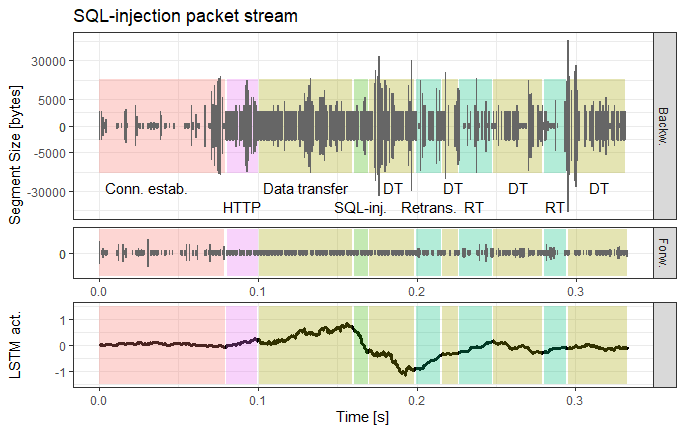
\includegraphics[width=0.8\textwidth]{images/LSTM_activation.png}
\caption{LSTM-output activation in dependence of connection phases. Depicted are packet segment streams and their respective sizes in the forward and backward direction, with different phases in the connection coloured and labelled. Below is the LSTM-ouput activation while processing the packet streams.}\label{fig:LSTM_act}
\end{figure}

The initially trained model performs relatively well, with an \textit{Area under curve} (AUC)-score\footnote{a measure describing the overall class separation of the model} of \textbf{0.981}, or a detection and false positive rate\footnote{tuned for the geometric mean} of \textbf{0.96\%} and \textbf{2.7\%}. However, these rates are still far from enabling operational deployment. Now suppose we want to improve these rates to both detect more SQL-injections and retain a lower false-positive rate.

We initially explore which type of connections are misclassified most often. For this, we perform a correlation analysis between the numeric or categoric labels available for the probing data, and the binary response whether the corresponding connection was misclassified. Unsurprisingly, the highest correlation to misclassification was measured for the conducted activity, with a particular attack scenario (19\% correlation) and connections with multiple GET-requests (11\% correlation) being confused most often. This was followed by the amount of simulated latency (12\% correlation), which we are now examining closer.



Fig. \ref{fig:LSTM_exp} depicts classification scores of connections in the probing data in dependence of the emulated network latency. The left panel depicts the scores for the initially trained model, which shows that while classification scores are well separated for lower congestion, increased latency in a connection leads to a narrowing of the classification scores, especially for SQL-injection traffic. Since there are no classification scores that reach far in the opposing area, we conclude that congestion simply makes the model lose predictive certainty. 
Increased latency can both increase variation in observed packet interarrival times (IATs), and lead to packet out-of-order arrivals and corresponding retransmission attempts. Both of these factors can decreases the overall sequential coherence for the model, i.e. that the LSTM-model loses context too quickly either due to increased IAT variation or during retransmission sequences. 


\begin{figure}
\centering
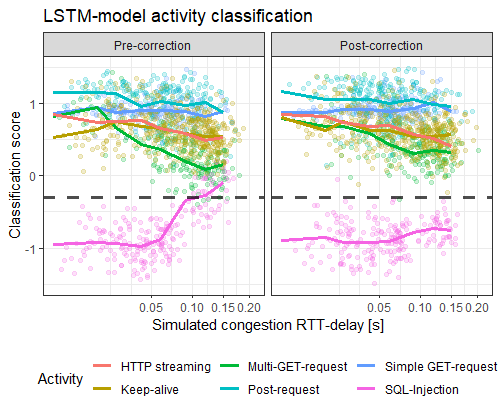
\includegraphics[width=0.8\textwidth]{images/LSTM_classi.png}
\caption{Scores for the LSTM-traffic classification model in dependence of simulated network congestion, along with the classification threshold. }\label{fig:LSTM_exp}
\end{figure}

To examine the exact effect of retransmission sequences on the model output, we generate two similar connections, where one connection is subject to moderate packet loss and reordering while the other is not. We then compare how the LSTM-output activation is affected by retransmission sequences. Fig. \ref{fig:LSTM_act} depicts the evolution the LSTM-output layer activation in dependence of difference connection phases. Initially the model begins to view the connection as benign when processing regular traffic, until the SQL-injection is performed. The model then quickly adjusts and provides a malicious classification after processing the injection phase and the subsequent data transfer. The negative output activation is however quickly depleted once the model processes a retransmission phase, and is afterwards not able to relate the still ongoing data transfer to the injection phase. When comparing this to the connection without retransmissions, we do not encounter this depletion effect, instead the negative activation persists after the injection phase.

We try to correct the existing model with a simple fix by excluding retransmission sequences from the model input data, both during training and classification. This leads to significantly better classification results during network latency, as visible in the right panel of Fig. \ref{fig:LSTM_exp}. SQL-injection scores are now far-less affected by congestion while scores for benign traffic are also less affected, albeit to a smaller degree.
The overall AUC-score for the model improves to \textbf{0.997} while tuned detection rates and false positives improved to \textbf{99.1\%} and \textbf{0.045\%}.


\section{Refining the notion of benign traffic for anomaly detection}\label{Sec:Refining}

Next, we show how ground-truth traffic information can help produce more coherent clusters and thus refine the benign traffic model in anomaly-detection. In particular, we will examine a 
simplified version of \textit{Kitsune} \cite{mirsky2018kitsune}, a recent deep learning anomaly-detection model based on stacked autoencoders. \textit{Kitsune's} AUC-scores surpassed those of other state-of-the-art methods for a variety of attacks, including various types of Botnet traffic and \textit{man-in-the-middle} attacks.

%for access attacks according to a survey by Nisioti et al. \cite{nisioti2018intrusion}.
The model takes connection packet streams as input, which are pushed through an artificial information bottleneck before reconstruction, which forces the model to learn and compress reoccurring traffic structures. The compressed connection representation is essentially a positional projection into a lower-dimensional vector space, where spatial boundaries around benign traffic can be drawn. For demonstration purposes, we use a widely-used clustering approach for anomaly-detection rather than \textit{Kitsune's} more complex ensemble method. 
%This allows us to project flows into a lower-dimensional vector space, where spatial boundaries around benign traffic can be drawn using clustering to identify anomalous traffic events. The model takes 102 flow summary statistics as input, which include features such as packet size and interarrival statistics, flag occurrencies, or number of flows in window. 
Here, anomalous outliers are detected using the Mahalanobis-distance of a projected connection from identified cluster centers. %The identified clusters therefore serve as structural enclosures of benign behaviour, with the cluster borders acting as separators to abnormal behaviours. 
Benign traffic should ideally be distributed evenly around the cluster centres to allow a tight borders and good separation from actual abnormal behaviour.

Unstructured datasets such as the CAIDA traffic traces assumably contain too much abnormal behaviour to train an anomaly-detection model, which is why we train the model on benign traffic from the CICIDS-17 \cite{sharafaldin2018toward} intrusion detection dataset (80\%). Again, we add 20\% probing traffic consists of HTTP, FTP, SSH, and SMTP communication, using a wide spectrum of settings for examination purposes. Attack data for the evaluation was again provided through the CICIDS-17 dataset, and includes access attacks such as SQL-injections or Brute-Forcing, as well as Mirai botnet traffic. We  train the model with in total 150,000 connections.

\subsection{Projection coherency evaluation}


Like many approaches that generate representations of benign traffic for anomaly detection, \textit{Kitsune} projects traffic events into a vector-space where traffic clusters and similarities become more apparent. In order for the projection to accurately capture important traffic structures, this projection should be consistent, i.e. traffic events with similar origins and characteristics should be projected to similar positions rather than be dispersed throughout the vector space \cite{hou2017deep}.

%Verifying the projection consistency of a model is not straightforward as usually no or not enough ground-truth information about different traffic characteristics is available to asses if the model is projecting similar traffic to dissimilar positions, or if the traffic just bears some dissimilar characteristics.

To verify the models projection consistency, we generate traffic from near-identical conditions to provide certainty on the expected traffic similarities. We generate a small dataset that consists of HTTP-requests, file-synchronisation, and Botnet communication. For each of the three traffic types we fix four settings that vary in the performed activity and network latency, with the traffic shaping described in Section \ref{Control} being held constant within each setting except for small variations in the transmitted message or file. Table \ref{Tab:Dataset} summarises the traffic for each setting. 

We verify if traffic samples within each group are projected to similar areas by measuring the average and maximum Mahalanobis-distance to quantify the overall dispersion of the samples. The results are displayed in Table \ref{Tab:Dataset} and depicted in Fig. \ref{fig:Subspace_disp}. The first thing to notice is that the model projects samples from each group within the same cluster, thus confirming the capture of a coarse traffic structure. When looking at the traffic dispersion and the corresponding Mahalanobis-distance measurements, we notice that the \textit{multi-request HTTP} traffic as well as the \textit{file-synchronisation} between mutliple computers is much further dispersed than in the other settings, especially when exposed to more latency. We also find that the corresponding dimension, $x_3$, with the most projected dispersion seems to be the same for each of the four settings. This suggests that the cause for the dispersion is the same for the different traffic types. 

We now focus on the influence of input features on the projected positions exclusively in the $x_3$-direction. Here, we can again perform a simple correlation analysis between different the input feature values and the corresponding $x_3$-value. We observe that the arrival time of packet bears the most correlation (5.4\%) for the selected settings. We also see that this influence is concentrated primarily on connections that are opened shortly after a previous connection, with the temporal separation between these two connections apparently being the primary cause for the spread on the $x_3$-axis. The connection interarrival times are naturally an important feature for \textit{Kitsune} to detect attacks such as \textit{Man-in-the-Middle}, which could explain the weight this feature plays in the projection process.

%look at the the influence of the individual flow features on projected position, we notice that even slight differences in the IAT of the preceding and the subsequent flow impacts the projected position quite strongly, which is why only the settings that generate multiple flows are affected.


\begin{figure}
\centering
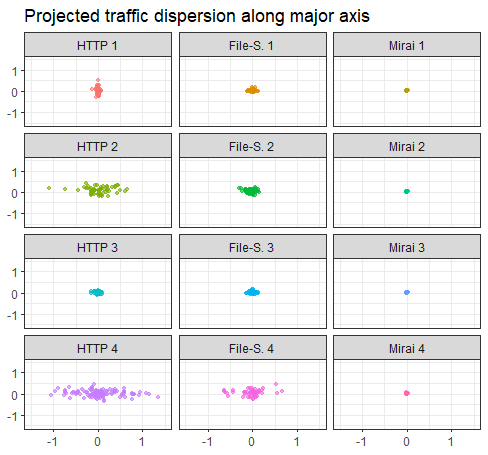
\includegraphics[width=0.7\textwidth]{images/traffic_dispersion.png}
\caption{Dispersion of projected traffic samples from each setting, plotted along the two most dispersed axes.}\label{fig:Subspace_disp}
\end{figure}

\section{Probing dataset}

We compiled and released a dataset suitable to quickly probe ML-model behaviour on a range of traffic characteristics. This dataset is designed to contain similar traffic as the CICIDS-17 and 18 datasets to allow probing of models trained on these \textcolor{red}{de-facto benchmark} datasets. 

\section{DetGen Architecture}

%DetGen is a container-based network traffic that we developed to enable repeatable, realistic, and flexible network experiments. DetGen is built on top of the widely used Mininet testbed \textcolor{red}{insert citation} and implements controllable communication scenarios for benign and attack traffic generation.

%\section{Background}\label{Sec:b8ackground}

\subsection{Design overview}

Detgen is a container-based network traffic generation framework that \textcolor{red}{dis.} % that we developed to enable repeatable, controllable, and \textcolor{red}{informative} network experiments. 
In contrast to the pool of programs running in a VM-setup, DetGen separates program executions and traffic capture into distinct containerised environments in order to shield the generated traffic from external influences and enable the fine-grained control of \textcolor{red}{traffic shaping factors}.

Traffic is generated from a set of scripted \textit{scenarios} (\textcolor{red}{give examples here}) that strictly control corresponding influence factors and offer the researcher to modify and label the conducted activity from a variety of \textcolor{red}{angles} and randomisations. %Containers communicate in a virtual network created with Mininet along with virtual software switches, Ethernet links, routers, and firewalls. %The network is then populated with containers ,which perform a variety of activities for traffic generation. The conducted activities are composed of scripted \textit{scenarios} (\textcolor{red}{give examples here}), but subject to a high degree of randomisation. The captured traffic events are labelled individually after the specific generating action.

\subsection{Containerization and activity isolation}
%\textcolor{red}{to do:need to improve}
Containers are standalone packages that contain an application along with all necessary dependencies using OS-level virtualization. In contrast with standard Virtual machines (VMs), containers forego a hypervisor and the shared resources are instead kernel artifacts that can be shared simultaneously across several containers, leading to minimal CPU, memory, and networking overhead \cite{kolyshkin2006virtualization}.



\begin{figure}
\centering
\begin{subfigure}[b]{0.48\textwidth}
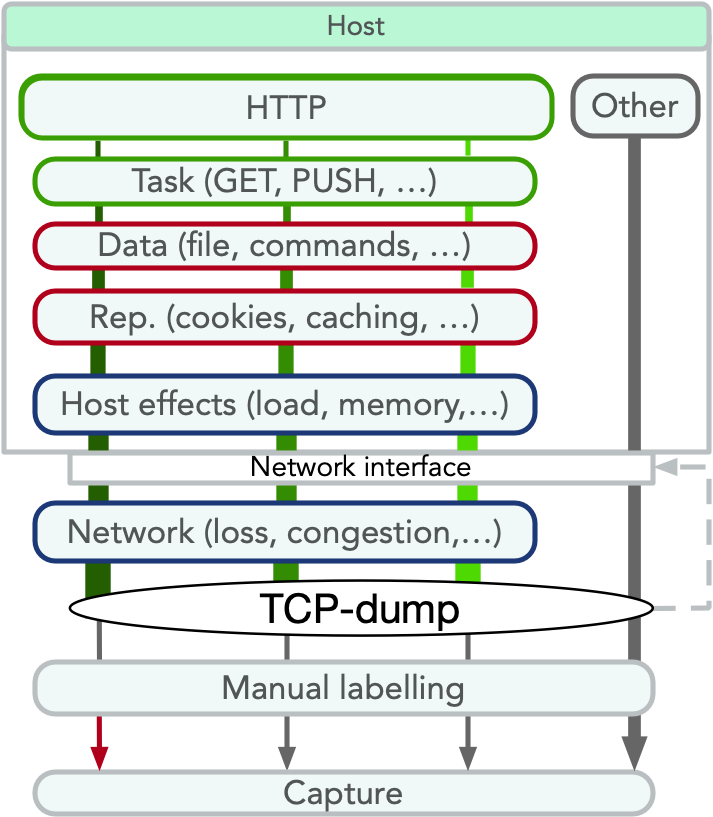
\includegraphics[width=\textwidth]{images/VM_setup_final.png}
\caption{Traditional capture setup}
\end{subfigure}
%~
\begin{subfigure}[b]{0.48\textwidth}
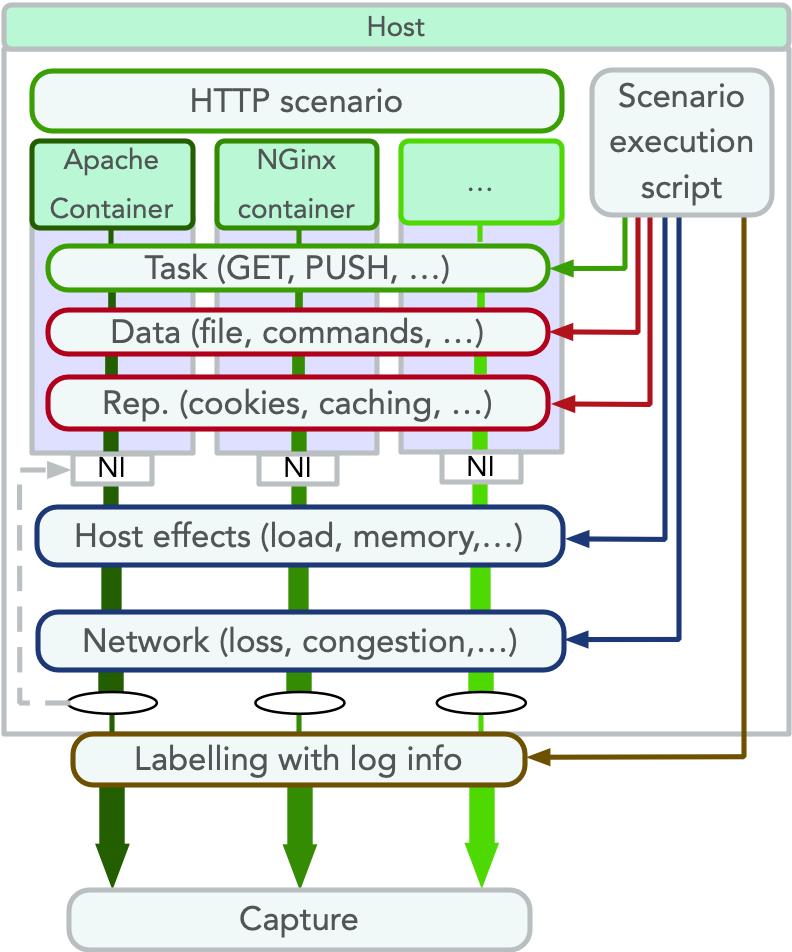
\includegraphics[width=\textwidth]{images/Docker_setup_final.png}
\caption{DetGen container setup}
\end{subfigure}
\caption{Design comparison of traditional NIDS-data-setups and our DetGen framework}
\end{figure}

%\textcolor{red}{Although this prevents the host environment from running different operating systems, containerization incurs minimal CPU, memory, and networking overhead whilst maintaining a great deal of isolation} \cite{kolyshkin2006virtualization}. 

Due to the separation of processes, containers provide significantly more isolation of programs from external effects than regular OS-level execution. This isolation enables us to monitor processes better and create more accurate links between traffic events and individual activities than on a virtual machine were multiple processes run in parallel, which can all generate traffic. The corresponding one-to-one correlation between processes and network traces allows us to produce labelled datasets with significantly more granular ground truth information.

\textcolor{red}{Insert some experimental result here}.

Containers are specified in an image-layer, which is unaffected during the container execution.
This allows containers to be run repeatedly whilst always starting from an identical state. In combination with the container isolation, this allows us to perform network experiments that can be easily reproduced by anyone on any plattform \textcolor{red}{insert citation}. 

%The container network interface provides the connection between a network namespace and the container runtimes. We want to \textcolor{red}{highlight} that multiple containers can share on network interface, which enables us to generate traffic from multiple applications over one network address in order to emulate \textcolor{red}{fully functional network hosts}.
 

\subsection{Activity generation}\label{Sec:Scenarios}

\subsubsection*{Scenario}
We define a \emph{scenario} as a series of Docker containers conducting a specific interaction, whereby all resulting network traffic is captured from each container's perspective. This constructs network datasets with total interaction capture, as described by Shiravi et al. \cite{shiravi2012toward}. Each scenario produces traffic from a specific setting with two (client/server) or more containers. 
%either a protocol, application or a series thereof. %Both benign and malicious activities are implemented as scenarios. 
Examples may include an FTP interaction, a music streaming application, an online login form paired with an SQL database, or a C\&C server communicating with an open backdoor. A full list of currently implemented scenarios can be found in Section \textcolor{red}{\ref{Sec:ExistScen}}.
Each scenario is designed to be easily started via a single script and can be repeated indefinitely without further instructions, therefore allowing the generation of large amounts of data.
Our framework is modular, so that individual scenarios are configured, stored, and launched independently. Adding or reconfiguring a scenario has no effect on the remaining framework.

When composing different settings, we most emphasised the inclusion of different \textbf{application layer protocols} such as HTTP or SSH, followed by the inclusion of different corresponding \textbf{applications} such as NGINX or Apache that steer the communication. We are currently aiming to also include options to use different \textbf{application layer implementations} such as TLS1.3 vs TLS1.2.

\subsubsection*{Task} \label{Sec:Subscenarios}

In order to provide a finer grain of control over the traffic to be generated, we create a catalogue of different tasks that allow the user to specify the manner in which a scenario should develop. The aim of having multiple tasks for each scenario is to explore the full breadth of a protocol or application's possible traffic behaviour. For instance, the SSH protocol can be used to access the servers console, to retrieve or send files, or for port forwarding, all of which may or may not be successful. It is therefore appropriate to script a number of tasks that cover this range of tasks.

To implement a catalogue of tasks, we first examine the functionality of the underlying protocol and scenario setting before proceeding to adding tasks to the catalogue. To explore the breadth of the corresponding traffic structures efficiently, we prioritise to add tasks that cover aspects such as direction of file transfers (e.g. GET vs POST for HTTP), the amount of data transferred (e.g. HEAD/DELETE vs GET/PUT), or the duration of the interaction (e.g. persistent vs non-persistent tasks) as much as possible. For each task, we furthermore add different failure options for the interaction to not be successful (e.g. wrong password or file directory). 

Since we always launch containers from the same state, we prevent traffic impact from \textbf{repetition effects} such as caching or known hosts. If an application provides caching possibilities, we implement this as an option to be specified before the traffic generation process.

%Subscenarios are specific to particular scenarios and can be specified when launching that scenario.

%The same applies to malicious activity. For instance, it would be naive for an SSH password bruteforcing scenario to always successfully guess a user's password. Instead, we include a second subscenario in which the password bruteforcer fails.

\subsubsection*{Input randomization}\label{Sec:randomsubscen}

Scripting activities that are otherwise conducted by human operators often leads to a loss of random variation that is normally inherent to the activity.
\textcolor{red}{As mentioned in Section \ref{Sec:problems}, the majority of successful FTP transfers in the CIC-IDS 2017 data consist of a client downloading a single text file.} In reality, file sizes, log-in credentials, and many other variables included in an activity are more or less drawn randomly, which naturally influences traffic quantities such as packet sizes or numbers.

We identify variable input parameters within scenarios and corresponding tasks and systematically draw them randomly from suitable distributions. Passwords and usernames, for instance, are generated as a random sequence of letters with a length drawn from a truncated Cauchy distribution, before they are passed to the corresponding container. Files to be transmitted are selected at random from a larger set of files, covering different sizes and file names.

%\begin{figure}
%\centering 
%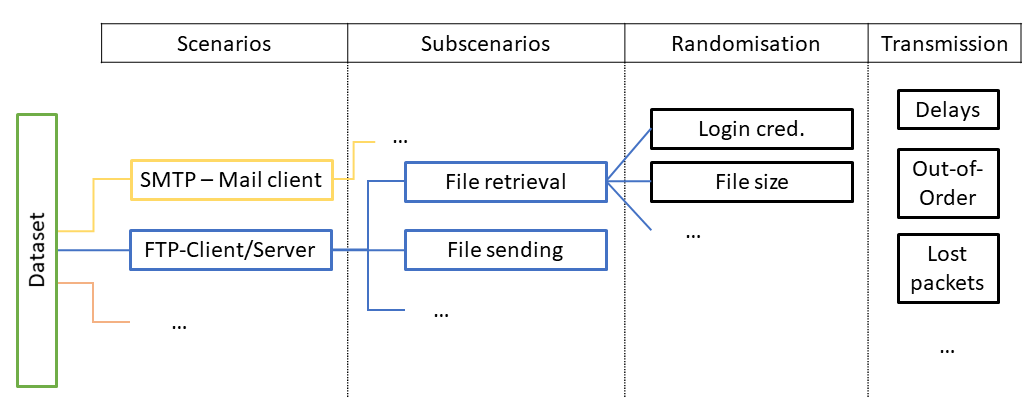
\includegraphics[width=0.5\textwidth]{images/scenario_branching.PNG}
%\caption{Visualization of the different levels at which traffic variation is introduced in DetGen.}
%\label{Fig:branching}
%\end{figure}



\subsection{Simulation of external influence}

\subsubsection*{Network effects}

Docker communication takes place over virtual bridge networks, 

Communication between containers takes place over a virtual Mininet bridge network, which provides far higher and more reliable throughput than in real-world networks. Gates and Warshavsky \cite{iperf} measured a bandwidth of over 90 Gbits/s without any lost packets using iPerf.8 This allows us to guarantee reliable and reproducible communication and thus remove external network effects on the captured traffic.

Virtual bridge networks furthermore enable us to retard and control the network reliability and congestion to a realistic level by using emulation tools. NetEm is an enhancement of the Linux traffic control facilities for emulating properties of wide area networks such as high latency, low bandwidth or packet corruption by adding delay, packet loss, duplication etc. to packets outgoing from a selected network interface \cite{hemminger2005network}.

We apply NetEm via a wrapping script to to the network interface of a given container, providing us with the flexibility to set each container's network settings uniquely. In particular, packet delays are drawn from a Paretonormal-distribution while packet loss and corruption is drawn from a binomial distribution, which has been found to emulate real-world settings well \cite{jurgelionis2011empirical}. Distribution parameters such as mean or correlation as well as available bandwidth can either be manually specified or drawn randomly before the traffic generation process.

%To retard the quality of the Docker network to realistic levels, we rely on emulation tools. As discussed in section \ref{sec:network}, Netem is a Linux command line tool that allows users to artificially simulate network conditions such as high latency, low bandwidth or packet corruption in a flexible manner.

%Although it is relatively straightforward to apply Netem commands to a Docker Bridge network, we decided not to invoke Netem in this manner as this would cause all network settings of all containers to be identical, such as all containers in a scenario having a latency of 50ms.  Instead, we developed a wrapping script that applies Netem commands to the network interface of a given container, providing us with the flexibility to set each container's network settings uniquely. This script randomizes the values of each parameter, such as packet drop rate, bandwidth limit, latency, ensuring that every run of a scenario has some degree of network randomization if desired.

\subsubsection{Host load}

We simulate excessive computational load on the host with the tool \emph{stress-ng}, a Linux workload generator. Currently, we only stress the CPU of the host, which is controlled by the number of workers spawned. Future work will also include stressing the memory of a system. We have investigated how stress on the network sockets affects the traffic we capture without any visible effect, which is why we omit this variable here.   

\subsection{Activity execution}

\subsubsection*{Execution script}

DetGen generates traffic through executing execution script that are specific to the particular scenario. The script creates the virtual network and populates it with the corresponding containers. The container network interfaces of the containers are then subjected to the NetEm chosen settings and the host is assigned the respective load, before the inputs for the chosen task are prepared and mounted to the containers. 

The user can then choose how long and how often to execute the scenario. Once the activity is terminated, the script takes down the network and containers, and repeats the process for the next repetition. Randomised settings are drawn anew for each repetition.

\subsubsection*{Labelling and traffic separation}

Each container network interface is hooked to a \emph{tcpdump}-container that records the packets that arrive or leave on this interface. Combined with the described process isolation, this setting allows us to exclusively capture traffic that corresponds to the conducted activity and exclude any background events. The captured traffic is then saved and labelled as a pcap-file. The execution script then stores all parameters (conducted task, mean packet delay,...) and descriptive values (input file size, communication failure, ...) for the chosen settings in a file along with the corresponding pcap-filename.

%\subsection{Network creation and population}

%To enable communication between containers, we build our framework on top Mininet \textcolor{red}{insert citation} to create virtual networks with customizable topology. 
%\textcolor{red}{A topology can be passed to a topology-creation wrapper in matrix form, with diagonal values representing the type of device (switch, container, router, ...), and off-diagonal indicating links}. This allows the import of larger, automatically generated topologies from tools such as \textcolor{red}{insert citation}. 

%\textcolor{red}{maybe something about subnets}. 

\subsection{Existing Scenarios}\label{Sec:ExistScen}

Our framework contains 29 scenarios, each simulating a different benign or malicious interaction. The protocols underlying benign scenarios were chosen based on their prevalence in existing network traffic datasets.%, a list of which can be found in the Appendix in Table \ref{tab:results-bro}. 
These datasets consist of common internet protocols such as HTTP, SSL, DNS, and SSH. According to our evaluation, our scenarios can generate datasets containing the protocols that make up at least $87.8\%$ (MAWI), $98.3\%$ (CIC-IDS 2017), $65.6\%$ (UNSW NB15), and $94.5\%$ (ISCX Botnet) of network flows in the respective dataset.
Our evaluation shows that some protocols that make up a substantial amount of real-world traffic are glaringly omitted by current synthetic datasets, such as BitTorrent or video streaming protocols, which we decided to include. 

\begin{table}
\begin{tabular}{l|l|r}
 \hline
 Name & Description & \#Ssc. \\
 \hline
 Ping & Client pinging DNS server & 1 \\
 Nginx & Client accessing Nginx server & 2\\
 Apache & Client accessing Apache server & 2\\
 SSH & Client communicating with & 5\\
 &SSHD server&\\
 VSFTPD & Client communicating with & 12\\
 &VSFTPD server&\\
% Scrapy & Client scraping website & 1 \\
 Wordpress & Client accessing Wordpress site & 5\\
 Syncthing& Clients synchronize files & 7\\
 &via Syncthing&\\
 mailx& Mailx instance sending & 5\\
 &emails over SMTP &\\
 IRC & Clients communicate via IRCd& 4\\
 BitTorrent & Download and seed torrents & 3 \\
 SQL & Apache with MySQL & 4\\
 NTP & NTP client & 2\\
 Mopidy & Music Streaming & 5\\
 RTMP & Video Streaming Server & 3\\
 WAN Wget & Download websites & 5 \\
\hline
\end{tabular}
%~
\begin{tabular}{l|l|r}
 \hline
 Name & Description & \#Ssc. \\
  \hline
 SSH B.force & Bruteforcing a password & 3\\
 &over SSH&\\
 URL Fuzz & Bruteforcing URL & 1\\
 Basic B.force & Bruteforcing Basic & 2\\
 &Authentication&\\
 Goldeneye & DoS attack on Web Server & 1\\
 Slowhttptest & DoS attack on Web Server & 4 \\
 Mirai & Mirai botnet DDoS & 3\\
 Heartbleed & Heartbleed exploit & 1\\
 Ares & Backdoored Server & 3\\
 Cryptojacking & Cryptomining malware & 1\\
 XXE & External XML Entity & 3\\
 SQLi & SQL injection attack & 2 \\
 Stepstone & Relayed traffic using & 2\\
 &SSH-tunnels&\\
 \hline
\end{tabular}
\caption{Currently implemented traffic scenarios along with the number of implemented subscenarios}
\label{tab:scen}
\end{table}

%\textcolor{red}{to do: explain more, maybe get one of the tables here if space}


In total, we produced 17 benign scenarios, each related to a specific protocol or application. Further scenarios can be added in the future, and we do not claim that the current list exhaustive. Most of these benign scenarios also contain many subscenarios where applicable.

The remaining 12 scenarios generate traffic caused by malicious behavior. These scenarios cover a wide variety of major attack classes including DoS, Botnet, Bruteforcing, Data Exfiltration, Web Attacks, Remote Code Execution, Stepping Stones, and Cryptojacking. 
Scenarios such as stepping stone behavior or Cryptojacking previously had no available datasets for study despite need from academic and industrial researchers.

%In particular the \emph{Cryptojacking} and the \emph{Stepstone} scenarios provide novel data of malicious behaviors that is currently unavaible to researchers. %\textcolor{red}{Should I mention that BT is very keen on the stepping stone scenario data, as there is none publicly available whatsoever?}

We provide a complete list of implemented scenarios in Table \ref{tab:scen}.




\section{Conclusions}\label{Sec:Conclusion}

In this paper, demonstrated the impact of traffic generation with extensive micro-structure control as well as detailed corresponding documentation on researchers ability to evaluate and understand network intrusion detection models. We implemented and trained two state-of-the art detection models before extensively probing their behaviour and limitations when encountering different traffic types. 

By using HTTP-traffic with congestion settings, we were quickly able to identify the inability of an LSTM-based classifier to handle traffic with significant retransmission rates, which enabled us to improve the model accordingly and increase detection performance by more than $2\%$. Similarly, the examination of projection consistency of a subspace-clustering method using traffic with artificially similar characteristics revealed an overly high sensitivity to flow interarrival times, while cluster-coherence could be increased significantly by identifying half-open connections that were dropped because of network failure as the source of overly dispersed traffic projections. 

These results have encouraged us to perform more deep-going probing of data-driven network intrusion detection models. We believe that in combination with strong NID-dataset, extensive model validation and corresponding development with targeted traffic samples might hold the key to reduce false positives of detection models to an acceptable rate, as well as help models replicate detection rates in practical settings.

\subsection{Difficulties and limitations}

%DetGen is building network traffic datasets from a small-scale level up by coalescing traffic from different fine-grained activities together. 
While the control of traffic micro-structures helps to understand models that perform on a packet- or connection-level, it does not replicate realistic network-wide temporal structures, such as port usage distributions or long-term temporal activity. The probing of models operating on aggregated, behavioural, or long-term features is therefore not effective, and variation in these quantities would have to be statistically estimated from other real-world traffic beforehand to allow our framework to emulate such behaviour reliably. Other datasets such as UGR-16 use this approach to fuse real-world and synthetic traffic and are currently better suited to build models of large-scale traffic structures.

Furthermore, while controlling traffic shaping factors artificially helps at identifying the limits and weak points of a model, it can exaggerate some characteristics in unrealistic ways and thus both affect the training phase of a model as well as tilt the actual detection performance of a model in either direction. Additionally, the artificial randomisation of traffic shaping factors can currently not generate the traffic diversity encountered in real-life traffic and thus only aid at exploring model limits extensively. The lack of realistic traffic heterogeneity however is at the moment significantly more pronounced in commonly used network intrusion datasets such as the CICIDS-17 dataset, where the vast majority of successful FTP-transfers consist of a client downloading a single text file that contains the Wikipedia page for ‘Encryption’.

\subsection{Future work}

\subsubsection*{Import of activity timeline}

The modelling and generation of computer network activity has been investigated extensively \textcolor{red}{(citations?)}, and tools to automatically generate realistic network activity streams 

we do not wish to \textcolor{red}{address} this topic here . Instead, our framework imports existing time-series of \textcolor{red}{host flow activity} to generate the corresponding communication. \textcolor{red}{give more info on flow generation tools} 

We transform existing network flow series into an activity timeline by \textcolor{red}{expand this}. We end up with an activity timeline that contains a set of timestamps along with the corresponding scenario and the source and destination host. 

%We paid meticulous attention to enable control over as many traffic impact factors as possible. However, DetGen is currently only offering insufficient control over underlying application-layer implementations such as TLS 1.3 vs 1.2. In theory, it should be unproblematic to provide containers with different implementations for each scenario to provide this control. However we faced difficulties to compile containers in a suitable manner and are currently investigating, how to improve DetGen on this shortcoming.

%Working with Docker containers can sometimes complicate the implementation of individual scenarios compared to working with VMs. Although several applications are officially maintained Docker containers that are free from major errors, many do not. For instance, in the \textit{BitTorrent} scenario, most common command line tools, such as \texttt{mktorrent}, \texttt{ctorrent} and \texttt{buildtorrent}, failed to actually produce functioning torrent files from within a container due to Docker's union filesystem. Furthermore, due to the unique way in which we are using these software packages, unusual configuration settings are sometimes needed. %As such, many 

%Lastly, capturing \texttt{.pcap}-files from each container can quickly exceed available disc space when generating traffic at scale. Depending on specific research requirements, it is advizable to add filtering or feature extraction commands to the scenario execution scripts to enable traffic preprocessing in real-time.




%We are grateful for our ongoing collaboration with our industry partners  on this topic area, who provided both ongoing support and guidance to this work. Discussions with them have helped reinforce the need for a better evaluation and understanding of the possibilities that new intelligent tools can provide.

%Full funding sources after currently blinded.

\bibliographystyle{abbrv}
 
\bibliography{../DetGen_ext}

%\appendix


\end{document}
